\documentclass{report}
\usepackage[T1]{fontenc} % Fontes T1
\usepackage[utf8]{inputenc} % Input UTF8
\usepackage[backend=biber, style=ieee]{biblatex} % para usar bibliografia
\usepackage{csquotes}
\usepackage[portuguese]{babel} %Usar língua portuguesa
\usepackage{blindtext} % Gerar texto automaticamente
\usepackage[printonlyused]{acronym}
\usepackage{hyperref} % para autoref
\usepackage{graphicx}
\usepackage{multirow}

\bibliography{bibliografia}


\begin{document}
%%
% Definições
%
\def\titulo{FPGA - Vending Machine}
\def\data{15/06/2021}
\def\autores{João Afonso Pereira Ferreira, \\ Guilherme Duarte Alves }
\def\autorescontactos{(103037) ferreiraafonsojoao@ua.pt, \\ (103185) guilherme.alves@ua.pt}
\def\versao{VERSAO 1}
\def\departamento{DETI - Departamento de Electrónica, Telecomunicações e Informática}
\def\empresa{Universidade de Aveiro(\emph{\href{https://www.ua.pt}{UA}})}
\def\logotipo{imagens/ua.pdf}
%
%%%%%% CAPA %%%%%%
%
\renewcommand{\contentsname}{Índice}
\begin{titlepage}

\begin{center}
%
\vspace*{50mm}
%
{\Huge \titulo}\\ 
%
\vspace{10mm}
%
{\Large \empresa}\\
%
\vspace{10mm}
%
{\LARGE \autores}\\ 
%
\vspace{30mm}
%
\begin{figure}[h]
\center
\includegraphics{\logotipo}
\end{figure}
%
\vspace{30mm}
\end{center}
%
\begin{flushright}
\versao
\end{flushright}
\end{titlepage}

%%  Página de Título %%
\title{%
{\Huge\textbf{Projeto Final nº 3 - Máquina de Vendas}}\\
{\LARGE\textit{Laboratórios de Sistemas Digitais}} \\ 
{\Large \departamento\\}
}
%
\author{%
    \autores \\ 
    \\\autorescontactos
}
%
\date{\data}
%
\maketitle

\pagenumbering{roman}

\tableofcontents
\listoftables     % descomentar se necessário
\listoffigures    % descomentar se necessário


%%%%%%%%%%%%%%%%%%%%%%%%%%%%%%%
\clearpage
\pagenumbering{arabic}

%%%%%%%%%%%%%%%%%%%%%%%%%%%%%%%%
\chapter{Introdução}
\label{chap.introducao}
Este projeto foi estritamente elaborado seguindo a linguagem de \textit{hardware}, de forma a simular, testar e modular com o auxílio de uma \textbf{FPGA} uma máquina automática de oferta de produtos, assumindo-se que esta disponibiliza 3 refrigerantes diferentes.
Neste relatório vão ser descritos as funcionalidades do sistema, arquitetura, as instruções para o bom desenvolvimento desta mesma máquina, assim como a conclusão, tendo sempre como base o \href{https://elearning.ua.pt/mod/folder/view.php?id=942630}{\textbf{guião}} de projetos finais fornecido pelos docentes da cadeira de Laboratórios de Sistemas Digitais (neste caso discute-se o projeto nº 3). 
%
\begin{center}
\LARGE\textbf{{Apresentação resumida da máquina}}
\end{center}
%
É pretendido que se implemente uma máquina de vendas de refrigerantes com memória capaz de:
%
\begin{itemize}
    \item guardar tanto o nome dos estados como comunicar ao utilizador o estado em que este se encontra;
    \item disponibilizar um \textit{Switch} que permita ao cliente escolher mais ou menos gelo usando as \textit{Keys} da FPGA(conceitos abordados posteriormente neste relatório)[\ref{chap.manual}];
    \item contar os tempos de cada operação programados pelos autores deste relatório.
\end{itemize} 
%
%table
%
\begin{table}
    \centering
    \begin{tabular}{|c|c|}
        \hline
        \textbf{Refrigerantes} & \textbf{Quantidade inicial de gelo} \\ \hline
        Sumo Pêssego (SPES) &\\
        Sumo Limão (SOLI)& 2\\ 
        Fanta (FAN) & \\
        \hline
    \end{tabular} \label{tabela}
    \caption{Refrigerantes disponíveis}
\end{table}

\begin{figure} 
    \centering
    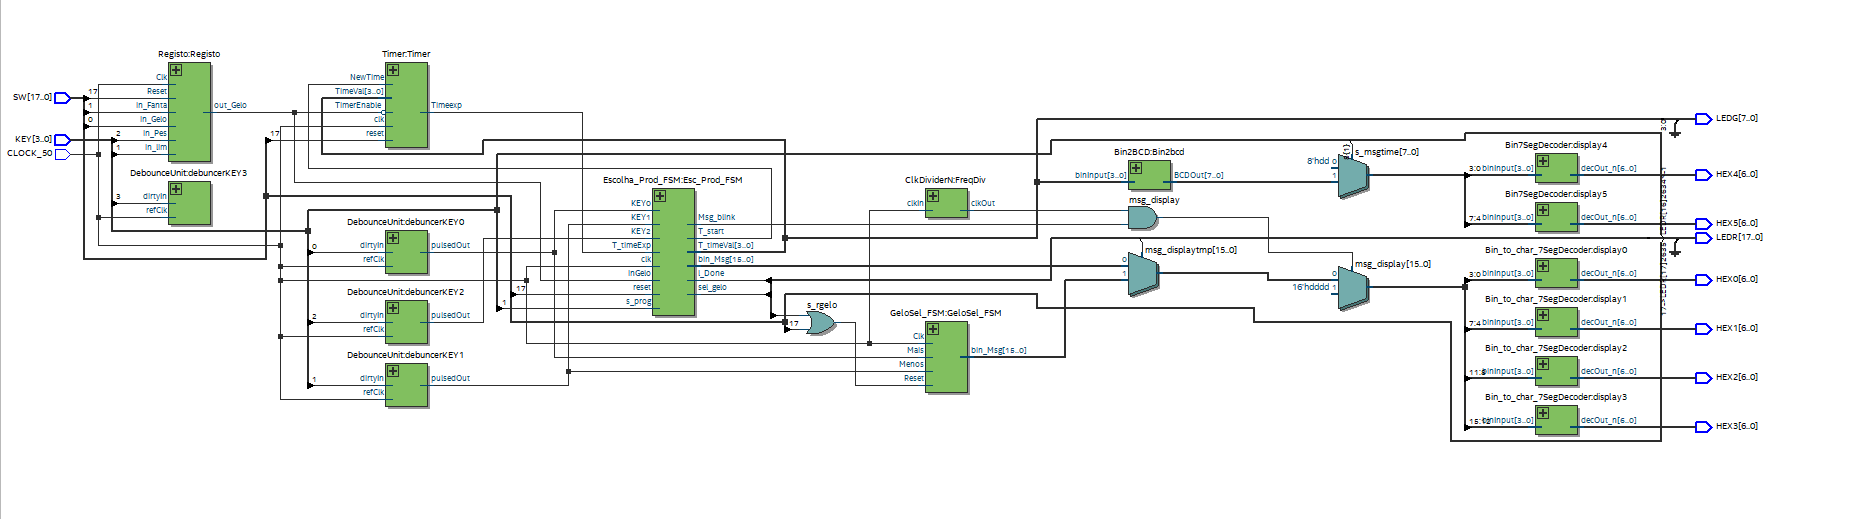
\includegraphics[width=\textwidth]{imagens/arch.png}
    \caption{\textit{Arquitetura detalhada do sistema}} \label{fig6:arch}
\end{figure}

\begin{figure} 
    \centering
    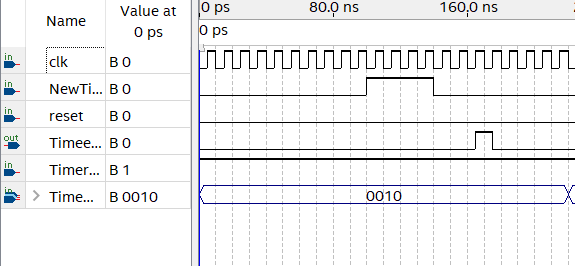
\includegraphics[width=\textwidth]{imagens/waveform.png}
    \caption{\textit{Funcionamento - Timer}} \label{fig6:timer}
\end{figure}

\chapter{Manual do Utilizador}
\label{chap.manual}
Após ligada a \textit{FPGA}~\cite{unknown2021}, esta apresenta uma mensagem nos \textit{displays} de 7 segmentos (HIHI) piscando à frequência de 6Hz - 1º estado para onde aponta a seta na fig.~\ref{fig6:fpga}. Passado 6 segundos ocorre a mudança de estado intitulado de \textit{OPTION}, resumindo "Escolha de refrigerante", este  apresentando também uma mensagem (EREF) (fig.~\ref{fig6:fpga}). A máquina permanecerá neste estado (OPTION) até nova indicação do utilizador por via dos 4 botões (\textit{KEY0, KEY1, KEY2 e KEY3}) que se encontram à direita dos "Switches" (interruptores localizados a baixo dos \textit{displays} de 7 segmentos), sendo que o KEY2 faz referência a Sumo Pêssego (SPES), KEY1 a Sumo Limão (SOLI) e KEY0 a Fanta (FAN)(fig.~\ref{refrig}). Após a escolha do produto desejado pelo cliente, o processo de preparação do produto demora cerca de 8s e, assim que concluída, é apresentada uma mensagem no \textit{display} de 7 segmentos (dOnE). Se pretender outro produto, basta aguardar cerca de 5 segundos para poder voltar a escolher mais um apetitoso refrigerante. Esta máquina, para o projeto em discussão, utiliza um sinal de clock de 50MHz para todos os componentes síncronos. É possível ainda considerar a proporção/quantidade de gelo que pretender na sua bebida, tendo como valor \textit{"default"} (base) 2 cubos de gelo, podendo ser alterada para mais ou menos entre os valores 0 e 5.


\begin{figure} 
    \centering
    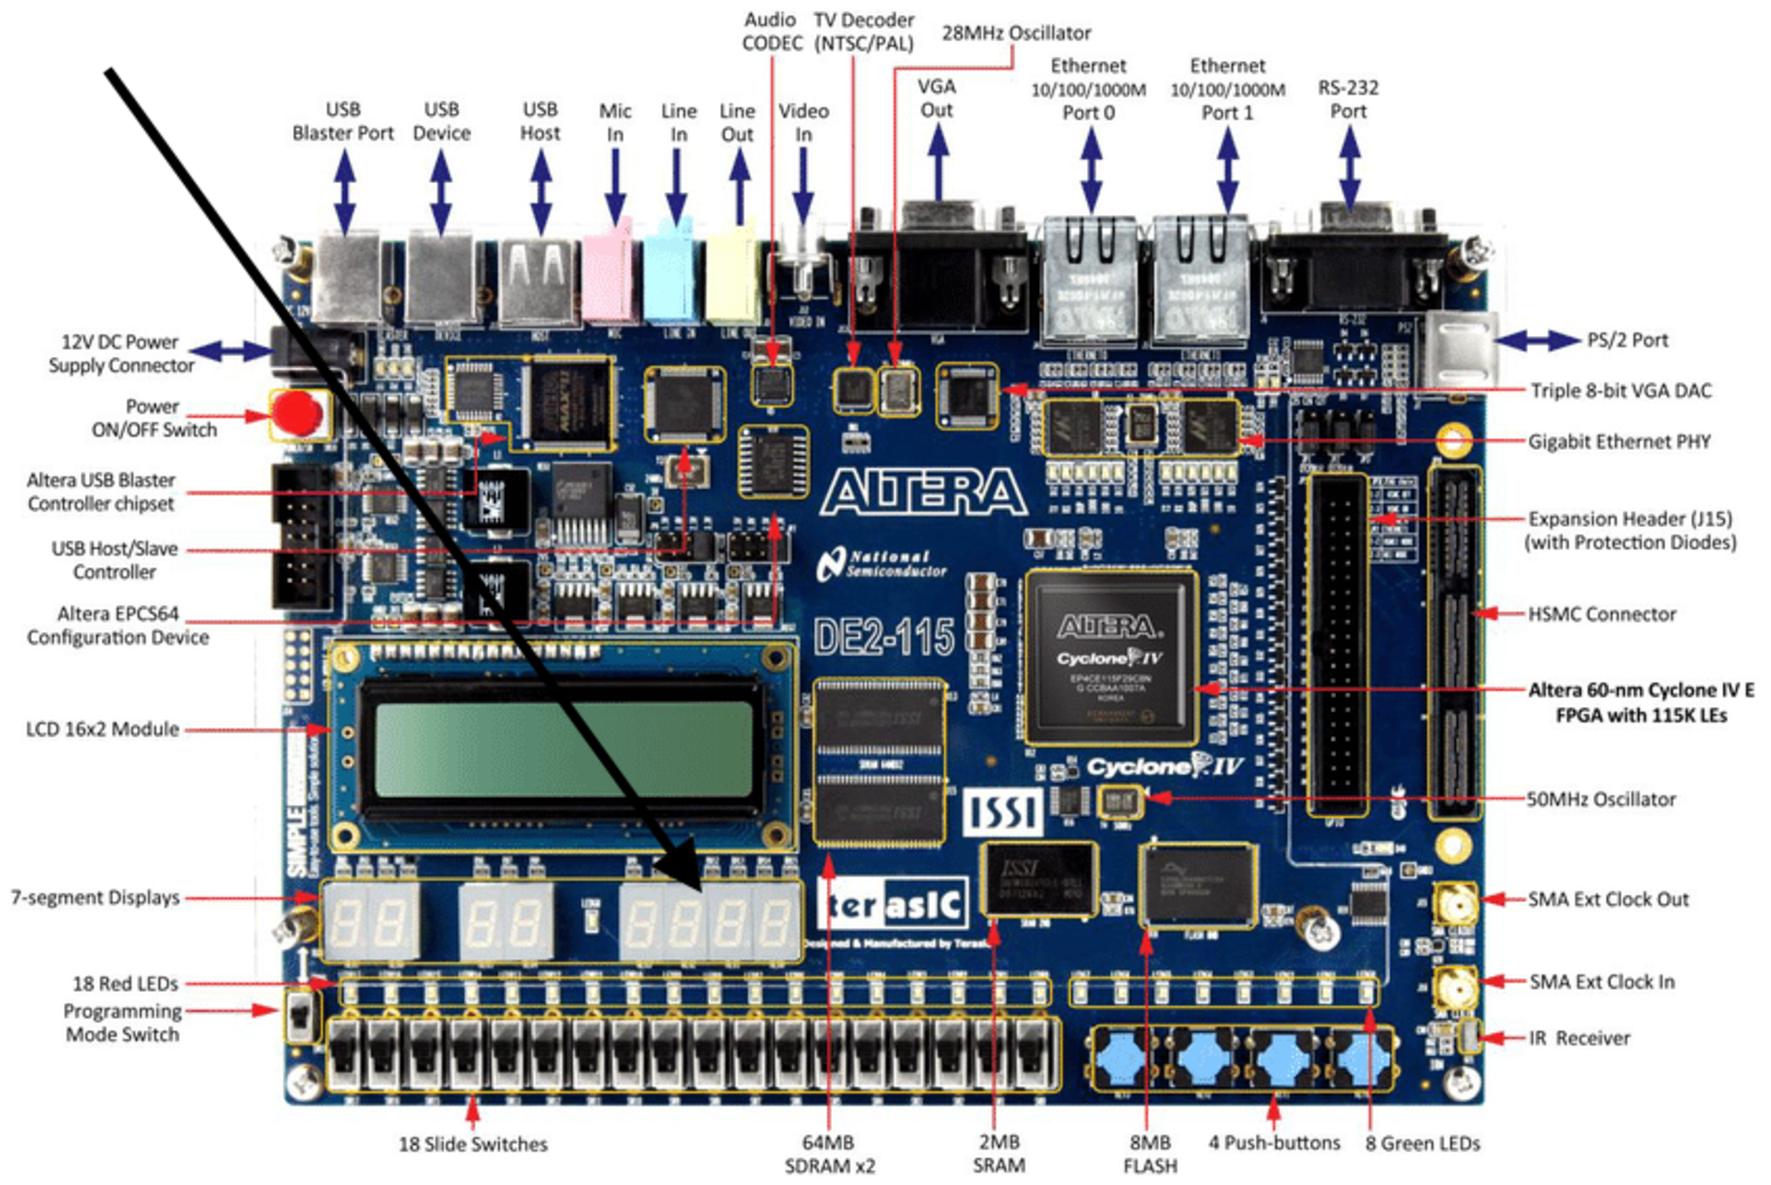
\includegraphics[width=\textwidth]{imagens/fpga.pdf}
    \caption{\textit{DE2-115 FPGA}} \label{fig6:fpga}
\end{figure}

  \begin{figure}[!h]
\centering
  $\vcenter{\hbox{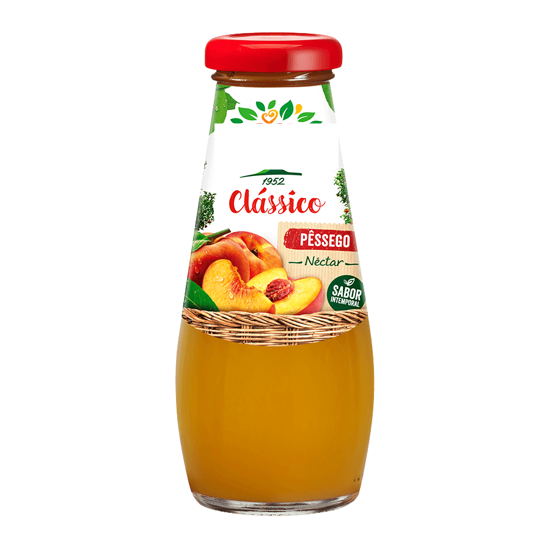
\includegraphics[height=3cm]{imagens/spes.png}}}$
  \qquad
  $\vcenter{\hbox{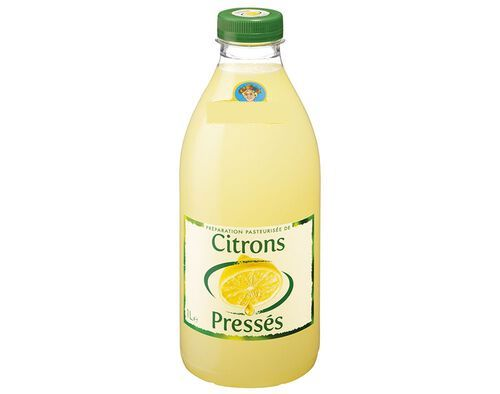
\includegraphics[height=3cm]{imagens/slim.jpg}}}$
  \qquad
  $\vcenter{\hbox{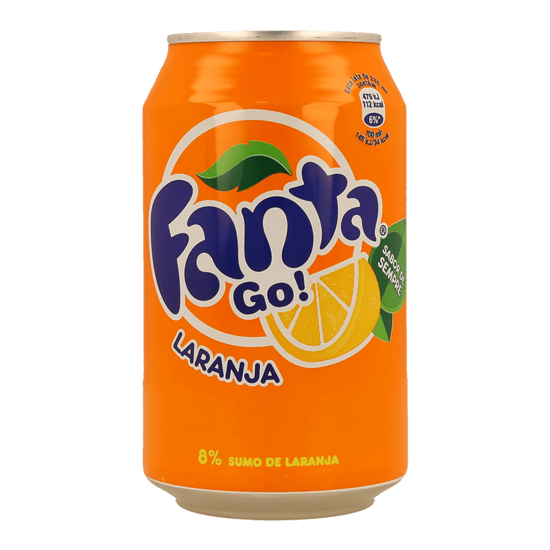
\includegraphics[height=3cm]{imagens/fan.png}}}$
\caption{refrigerantes ordenados (SPES, SOLI, FAN)}
\label{refrig}
\end{figure}


\chapter{Metodologia}
\label{chap.metodologia}
\section{Implementação}
A implementação deste trabalho tem como base registos, \textit{timer} e máquinas de estados finitos \cite{ericmccreath2008} seguido de simulação, modulação, teste e de acordo com as fases a seguir apresentadas e detalhadas.

\subsection{Fase 1}
Implementação da máquina de refrigerantes de acordo com as especificações descritas acima sem o modo “Escolha cubos de gelo”. O cliente escolhe o refrigerante e assim que estiver pronto, sai.

\subsection{Fase 2}
Após concluída a fase 1, esta fase deverá ser implementado o modo “Escolha cubos de gelo”. Dever ser possível aumentar ou diminuir o número de cubos de gelo a adicionar. A diminuição do número de cubos deverá ser feito através da entrada KEY0 e o aumento através da KEY1. Por defeito deverá estar configurado para 2 cubos de gelo isto é, após ativar este modo deverá parecer “00” nos \textit{Displays} de 7 segmentos. Os 4 Displays apagados significa refrigerante sem gelo.

\subsection{Fase 3}
Confirmar se a máquina deve utilizar um sinal de clock de 50MHz para todos os componentes síncronos.

\subsection{Fase 4}
Verificar a existência de um botão de \textit{RESET}(SW(17)) global que coloca a máquina nas condições iniciais.

\chapter{Conclusões}
\label{chap.conclusao}
Com este trabalho, foi possível expandir os nossos conhecimentos e horizontes acerca de placas \textbf{FPGA} e o seu funcionamento, bem como a linguagem de \textit{hardware} \textbf{VHDl}. Foi possível constatar o bom funcionamento da máquina de vendas de refrigerantes, de acordo, com as indicações propostas pelos professores. As fases anteriormente referidas foram cumpridas com sucesso, obtendo uma máquina que segue quase todos os requisitos.

\chapter*{Contribuições dos autores e auto avaliação}
Ambos os autores deste trabalho contribuíram para a realização do mesmo, destacando-se o Guilherme Alves. Desta forma, Guilherme alves com 60\% (17/20 valores) e João Ferreira com 40\% (15/20 valores).

%%%%%%%%%%%%%%%%%%%%%%%%%%%%%%%%%
\printbibliography

\end{document}
